% ★★ 中档
\newcommand{\qConicHardEllipseSlopeStem}{
已知椭圆 $C: \frac{x^2}{2} + y^2 = 1$．过点 $P(0, -2)$ 的直线 $l: y = kx + m$ 与椭圆 $C$ 交于不同的两点 $A, B$．设直线 $PA, PB$ 的斜率分别为 $k_{PA}, k_{PB}$．若 $k_{PA} + k_{PB} = 0$，求证：直线 $l$ 恒过定点，并求出该定点坐标．
}
\newcommand{\qConicHardEllipseSlopeFigure}{
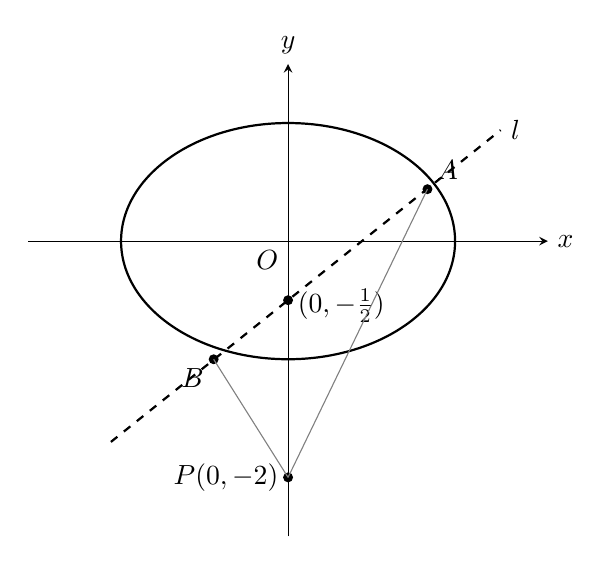
\begin{tikzpicture}[scale=1.5, >=stealth]
  % Axes
  \draw[->] (-2.2,0) -- (2.2,0) node[right] {$x$};
  \draw[->] (0,-2.5) -- (0,1.5) node[above] {$y$};
  \node[below left] at (0,0) {$O$};
  
  % Ellipse
  \draw[thick] (0,0) ellipse (1.414 and 1.0);
  
  % Point P
  \coordinate (P) at (0, -2.0);
  \fill (P) circle (1.2pt) node[left] {$P(0, -2)$};
  
  % Line l: y = 0.5x - 0.5 (passes through (0, -0.5) and has k=0.5)
  \coordinate (Fixed) at (0, -0.5);
  \fill (Fixed) circle (1.2pt) node[right, yshift=-2pt] {$(0, -\frac{1}{2})$};
  
  % A and B are intersections of y = 0.8x - 0.5 with x^2/2 + y^2 = 1
  % x^2/2 + (0.8x - 0.5)^2 = 1 => 0.5x^2 + 0.64x^2 - 0.8x + 0.25 = 1 => 1.14x^2 - 0.8x - 0.75 = 0
  % roots approx x1 = 1.23, y1 = 0.48; x2 = -0.53, y2 = -0.92
  \coordinate (A) at (1.18, 0.44);
  \coordinate (B) at (-0.63, -1.0);
  \fill (A) circle (1.2pt) node[above right] {$A$};
  \fill (B) circle (1.2pt) node[below left] {$B$};
  
  % Lines
  \draw[thick, dashed] (-1.5, -1.7) -- (1.8, 0.94) node[right] {$l$};
  \draw[thin, gray] (P) -- (A);
  \draw[thin, gray] (P) -- (B);
\end{tikzpicture}
}
\newcommand{\qConicHardEllipseSlopeAnswer}{
证明见解析．直线 $l$ 恒过定点 $(0, -\frac{1}{2})$．
}
\newcommand{\qConicHardEllipseSlopeSolution}{
\begin{proof*}
设直线 $l$ 的方程为 $y = kx + m$，其一般式为 $kx - y + m = 0$，对应硬解系数为 $A=k, B=-1, C=m$．\\
椭圆 $C: \frac{x^2}{2} + y^2 = 1$，对应半轴平方参数为 $a^2=2, b^2=1$．\\
此时统一分母为 $D = A^2a^2 + B^2b^2 = 2k^2 + 1$．\\
联立直线与椭圆的方程，应用硬解定理可直接写出消元后的一元二次方程：
\[
(2k^2 + 1)x^2 + 4kmx + 2(m^2 - 1) = 0
\]
因为直线与椭圆交于不同的两点 $A(x_1, y_1), B(x_2, y_2)$，根据相交充要条件 $D > C^2$，即 $2k^2 + 1 > m^2$，所以判别式应满足：
\[
\Delta = (4km)^2 - 8(2k^2 + 1)(m^2 - 1) = 8(2k^2 - m^2 + 1) > 0
\]
由硬解定理直接写出交点的横坐标韦达公式，省去了常规消元展开合并的计算量：
\[
x_1 + x_2 = -\frac{2ACa^2}{D} = -\frac{4km}{2k^2 + 1},\qquad x_1x_2 = \frac{a^2(C^2 - B^2b^2)}{D} = \frac{2(m^2 - 1)}{2k^2 + 1}
\]
由点 $P(0, -2)$，可知直线 $PA, PB$ 的斜率存在，且：
\[
k_{PA} + k_{PB} = \frac{y_1 - (-2)}{x_1} + \frac{y_2 - (-2)}{x_2} = \frac{y_1 + 2}{x_1} + \frac{y_2 + 2}{x_2} = 0
\]
将 $y_1 = kx_1 + m, y_2 = kx_2 + m$ 代入上式中整理：
\[
\frac{kx_1 + m + 2}{x_1} + \frac{kx_2 + m + 2}{x_2} = 2k + (m + 2)\left(\frac{1}{x_1} + \frac{1}{x_2}\right) = 2k + (m + 2)\frac{x_1 + x_2}{x_1x_2} = 0
\]
将韦达定理结果代入上式分式中：
\[
\frac{x_1 + x_2}{x_1x_2} = \frac{-\frac{4km}{2k^2 + 1}}{\frac{2(m^2 - 1)}{2k^2 + 1}} = -\frac{2km}{m^2 - 1}
\]
从而：
\[
2k + (m + 2)\left(-\frac{2km}{m^2 - 1}\right) = 2k\left(1 - \frac{m(m + 2)}{m^2 - 1}\right) = 2k\left(\frac{m^2 - 1 - m^2 - 2m}{m^2 - 1}\right) = 2k\left(\frac{-2m - 1}{m^2 - 1}\right) = 0
\]
当 $k = 0$ 时，直线 $l: y = m$ 平行于 $x$ 轴，此时 $A, B$ 关于 $y$ 轴对称，$x_1 + x_2 = 0$，且 $y_1 = y_2 = m$．\\
此时 $k_{PA} = \frac{m+2}{x_1}, k_{PB} = \frac{m+2}{-x_1} = -k_{PA}$，所以对任意 $m \in (-1, 1)$，恒有 $k_{PA} + k_{PB} = 0$，此时无法唯一确定 $m$．\\
由于直线 $l$ 变动，故对于 $k \neq 0$ 的情况，必须满足：
\[
-2m - 1 = 0 \implies m = -\frac{1}{2}
\]
当 $m = -\frac{1}{2}$ 时，代入判别式条件：$2k^2 + 1 > \frac{1}{4}$ 恒成立，且 $m^2 - 1 = -\frac{3}{4} \neq 0$，满足题意．\\
此时直线 $l$ 的方程为 $y = kx - \frac{1}{2}$，恒过定点 $(0, -\frac{1}{2})$．
\end{proof*}
}
\newcommand{\qConicHardEllipseSlopeDiagnosis}{
\errortag{特殊情况漏失} 学生在化简 $2k\left(\frac{-2m-1}{m^2-1}\right) = 0$ 时容易直接得出 $-2m-1=0$，忽略了 $k=0$ 时斜率积本来就为 $0$ 的特殊性．在解答题中应分类讨论或明确指出 $k \neq 0$ 的条件，否则扣分．\\
\errortag{代数运算繁琐} 部分学生不擅于提取公因式 $2k$，而是将 $y_1, y_2$ 展开直接通分，导致计算量翻倍，极易在通分中计算出错．
}
